\documentclass[12pt]{article}

\usepackage{caption}
\usepackage{changepage} % adjustwidth
\usepackage{xcolor}
\usepackage{float}
\usepackage{graphicx}
\usepackage{fancyhdr}
\usepackage{listings} % Code listings
\usepackage{multicol}
\usepackage{multirow}

\usepackage[utf8]{inputenc}
\usepackage{setspace}

\usepackage[dvips,letterpaper,margin=1in]{geometry}

\setlength{\parindent}{15pt}
\setlength{\headheight}{15pt} % fancyhdr wants at least 14.5pt

% Header
\pagestyle{fancy}
\lhead{K3 Migration to Red Hat Real-Time Linux}
\rhead{August 28, 2020}
\renewcommand{\headrulewidth}{0.4pt}
\renewcommand{\footrulewidth}{0.4pt}

% Start document
\begin{document}

%%%%%%%%%%%%%%%%%%%% Title Page %%%%%%%%%%%%%%%%%%%%%%%%
\thispagestyle{empty}
\begin{titlepage}
\begin{center}
        \vspace*{1cm}

        \LARGE{Ku Band Radio Frequency System Version 3 (K3) \\
        Migration from Concurrent RedHawk Linux to \\
        Red Hat Real-Time Linux}

        \vspace{0.5cm}
        \LARGE
        % Subtitle

        \vspace{1.5cm}

        \normalsize

        John Jesus \\
        August 28, 2020

        \vfill



        \vspace{0.8cm}




\end{center}
\end{titlepage}

\tableofcontents
\newpage

%%%%%%%%%%%%%%%%% Scope %%%%%%%%%%%%%%%%%%%%%%%%
%
\section{Scope}
\subsection{Identification}
This document is a Raytheon internal document analyzing an opportunity to change the version of Linux operating system used in the Ku Band Radio Frequency System (KRFS) Version 3 (K3).

\subsection{System overview}
KRFS is a radar system that supports the counter- rocket, artillery, and mortar (CRAM) mission.
KRFS has four radar apertures each operating as an Active Electronically
Scanned Array (AESA).  Each aperture has its own receiver/exciter and signal processing
subsystem called the Array Backend Electronics Unit (ABEU).  The arrays are arranged to
provide 360 degree coverage in azimuth and horizon to 90-degree coverage in elevation.

\begin{figure}[H]
    \begin{center}
    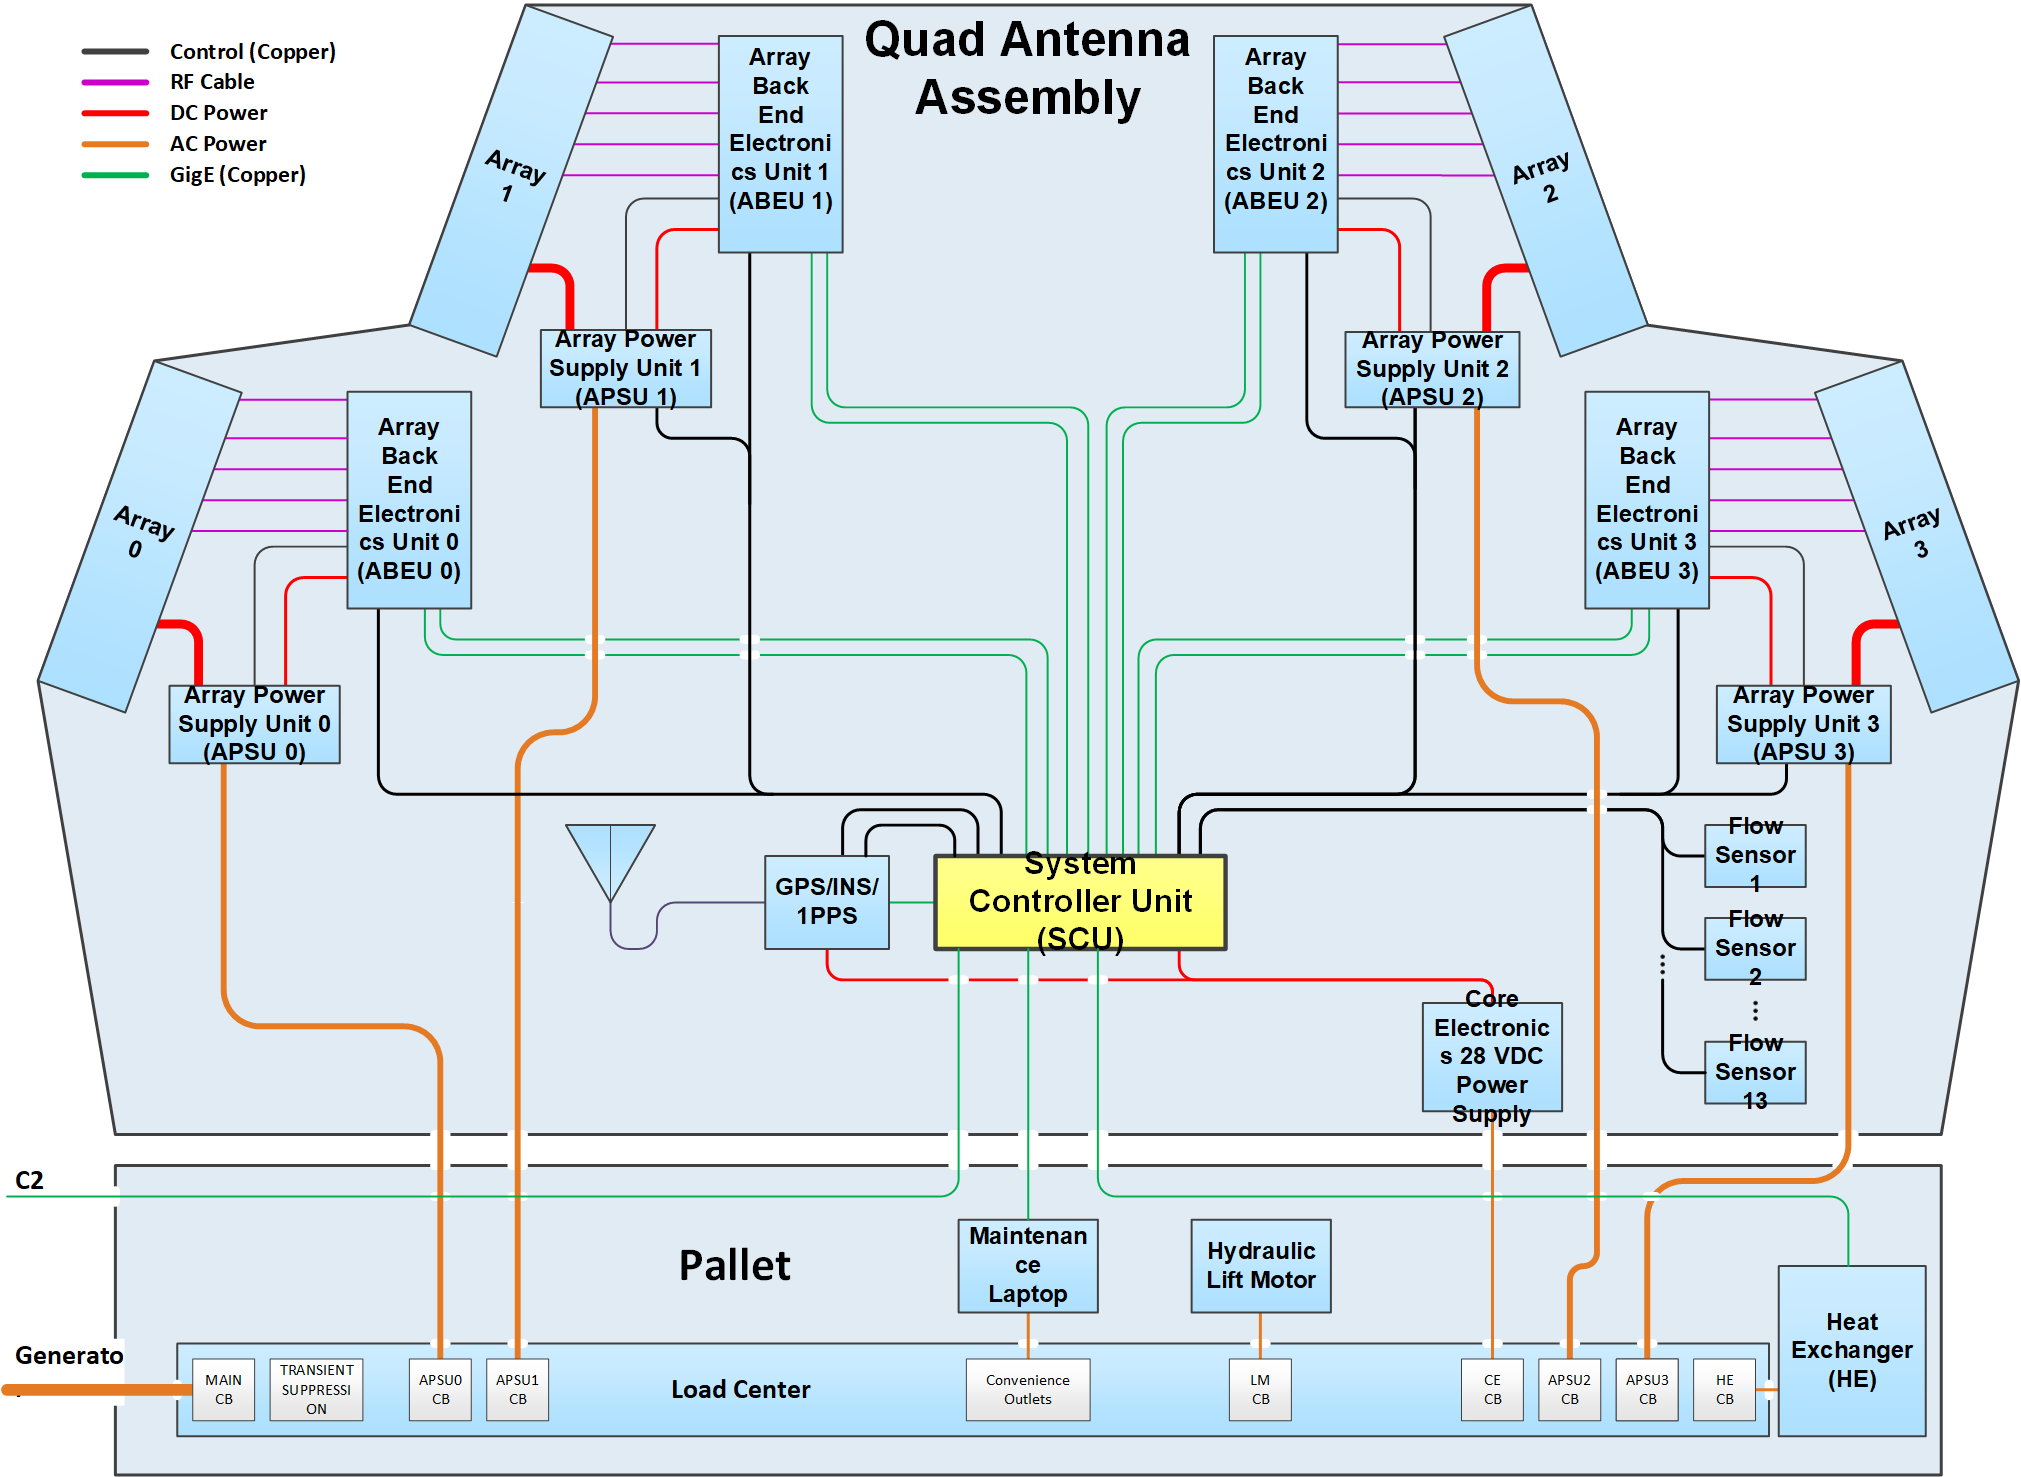
\includegraphics[width=1.0\textwidth]{img/k3}
    \caption{K3 Radar System}
    \label{fig:k3}
    \end{center}
\end{figure}

The System Controller Unit (SCU) is a 3-U VPX/VME shelf with commercial-off-the-self (COTS)
cards and one custom card assembly (CCA).  The SCU is the central controller for the radar system,
and the main control software within the SCU runs in its SBC card (Figure \ref{fig:scu}).

\begin{figure}[H]
    \begin{center}
    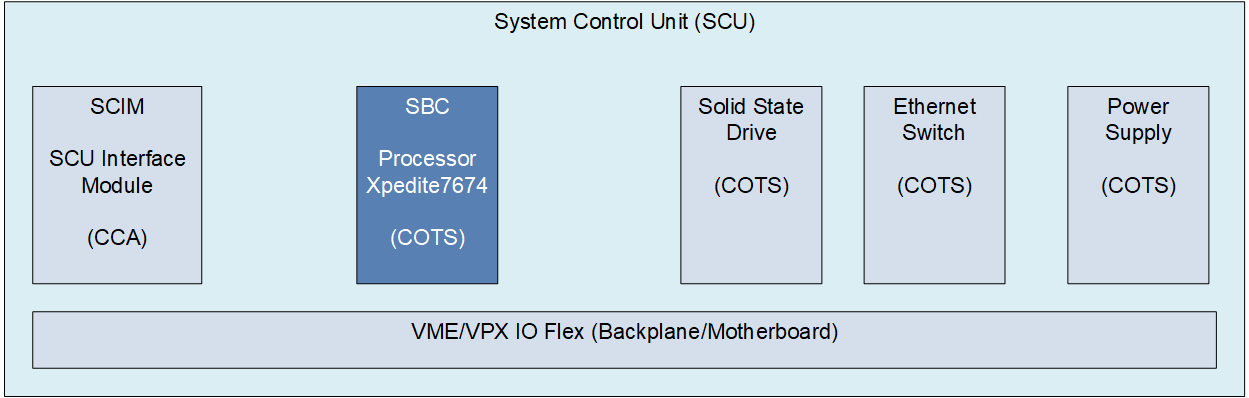
\includegraphics[width=1.0\textwidth]{img/scu}
    \caption{The SBC card in the SCU}
    \label{fig:scu}
    \end{center}
\end{figure}

In KRFS K2, the SBC Processor is a Extreme Engineering (XES) Xpedite7672 card based on the Xeon-D
System-on-a-Chip (SOC) running the Linux operating system.
In KRFS K3, the SBC Processor is a very similar Extreme Engineering (XES) Xpedite7674 card also based on the Xeon-D SOC and running the Linux operating system.

\subsection{Linux operating system}

\subsubsection{Linux operating system in KRFS K2}

\subsubsection{Linux operating system in KRFS K3}


\subsection{Document purpose}
To integrate NE software, we need to be able to build Linux from source.  NE currently uses Red Hat Real-Time.  We use Red Hawk from Concurrent RTI.  NE builds from source using tools from Red Hat.  We do not build from source.

Produce a document that helps us decide how to get our Linux image created.


\subsection{Document overview}
The structure of this document:

\begin{enumerate}
    \item Document scope (this section)
    \item References
    \item Real-time features from RedHawk in current K2 software
    \item Creating the Linux operating system image
    \item Hardening the Linux operating system image
    \item Migrating to Red Hat Real-Time in K3
\end{enumerate}



%%%%%%%%%%%%%%%%% References %%%%%%%%%%%%%%%%%%%%%%%%
%
\section{References}

\begin{enumerate}
    \item RedHawk Linux Users Guide 0898004-780 (Concurrent Computer Corporation, March 2016) \label{ref:red_hawk_guide}
    \item RedHawk Architect Users Guide  0898601-7.2-1 (Concurrent Computer Corporation, December 2016) \label{ref:architect}
\end{enumerate}


%%%%%%%%%%%%%%%%% RedHawk Features %%%%%%%%%%%%%%%%%%%%%%%%
%
\section{Real-time features from RedHawk}
\label{sec:redhawk_features}

\begin{table}[H]
    \captionsetup{width=.9\linewidth}
    \caption{RedHawk real-time feature list}
    \resizebox{\textwidth}{!}{%
    \begin{tabular}{p{3.0in}p{1.0in}p{3.0in}}
    \hline
        Feature & Used & Description \\
    \hline
        Processor Shielding & Yes & cpuset \\
        Processor Affinity & Yes & set affinity \\
    \hline
User-level Preemption Control & No & non-preempt spinlock, resched\_cntl \\
Fast Block/Wake Services & No & pw\_wait \\
RCIM Driver & No & 400ns clock source \\
Frequency-Based Scheduler & No & \\
/proc Modifications & No & (same as usermap) \\
Kernel Trace Facility & No & (Nighthawk) \\
ptrace Extensions & No & (Nighthawk usermap) \\
Kernel Preemption & (built-in) &  \\
Real-Time Scheduler & (built-in) & fixed-length context switch, non-CFS (Completely Fair Scheduler) \\
Low Latency Enhancements & (built-in) & tunable kernel spinlock \\
Priority Inheritance & (built-in) & \\
High Resolution Process Accounting & No & \\
Capabilities Support & (built-in) & \\
Kernel Debuggers & (built-in) & \\
Kernel Core Dumps/Crash and Live Analysis & (built-in) & \\
User-level Spin Locks & No & \\
usermap and /proc mmap & No & \\
Hyper-threading & (built-in) & tunable \\
XFS Journaling File System & No & \\
    \hline
    \end{tabular}%
    }
    \label{tab:redhawk_features}
\end{table}


%%%%%%%%%%%%%%%%% Image creation %%%%%%%%%%%%%%%%%%%%%%%%
%
\section{Creating the Linux operating system image}
\label{sec:image_creation}



%%%%%%%%%%%%%%%%% Hardening %%%%%%%%%%%%%%%%%%%%%%%%
%
\section{Hardening the Linux operating system image}
\label{sec:image_hardening}



%%%%%%%%%%%%%%%%% Migrating to Red Hat %%%%%%%%%%%%%%%%%%%%%%%%
%
\section{Migrating to Red Hat Real-Time in K3}
\label{sec:redhat_migration}


\end{document}

